%\documentclass[11pt,a4paper]{article}
\newcommand{\elemof}{\in\,}

\documentclass{sig-alternate-05-2015}
\usepackage[latin1]{inputenc}
\usepackage{amsmath}
\usepackage{amsfonts}
\usepackage{amssymb}
\usepackage{subfigure}
\usepackage{graphicx}
\usepackage{url}
\usepackage[linesnumbered,ruled]{algorithm2e}

% Copyright
\setcopyright{acmcopyright}
%\setcopyright{acmlicensed}
%\setcopyright{rightsretained}
%\setcopyright{usgov}
%\setcopyright{usgovmixed}
%\setcopyright{cagov}
%\setcopyright{cagovmixed}

\begin{document}
\conferenceinfo{GECCO'17,} {July 15-19, 2017, Berlin, Germany}
\CopyrightYear{2017}
\crdata{TBA}
\clubpenalty=10000
\widowpenalty = 10000

\title{Evolving a Real-time Evacuation for Urban Disaster Management}

%
% You need the command \numberofauthors to handle the 'placement
% and alignment' of the authors beneath the title.
%
% For aesthetic reasons, we recommend 'three authors at a time'
% i.e. three 'name/affiliation blocks' be placed beneath the title.
%
% NOTE: You are NOT restricted in how many 'rows' of
% "name/affiliations" may appear. We just ask that you restrict
% the number of 'columns' to three.
%
% Because of the available 'opening page real-estate'
% we ask you to refrain from putting more than six authors
% (two rows with three columns) beneath the article title.
% More than six makes the first-page appear very cluttered indeed.
%
% Use the \alignauthor commands to handle the names
% and affiliations for an 'aesthetic maximum' of six authors.
% Add names, affiliations, addresses for
% the seventh etc. author(s) as the argument for the
% \additionalauthors command.
% These 'additional authors' will be output/set for you
% without further effort on your part as the last section in
% the body of your article BEFORE References or any Appendices.

\numberofauthors{5} %  in this sample file, there are a *total*
% of EIGHT authors. SIX appear on the 'first-page' (for formatting
% reasons) and the remaining two appear in the \additionalauthors section.
%

\author{
% You can go ahead and credit any number of authors here,
% e.g. one 'row of three' or two rows (consisting of one row of three
% and a second row of one, two or three).
%
% The command \alignauthor (no curly braces needed) should
% precede each author name, affiliation/snail-mail address and
% e-mail address. Additionally, tag each line of
% affiliation/address with \affaddr, and tag the
% e-mail address with \email.
%
% 1st. author
\alignauthor
Keith J. Drew\\
\affaddr{University of Idaho}\\
\affaddr{895 Perimeter Drive}\\
\affaddr{Moscow, Idaho 83844}\\
\email{keithd@vandals.uidaho.edu}
% 2nd. author
\alignauthor
Robert B. Heckendorn\\
\affaddr{University of Idaho}\\
\affaddr{895 Perimeter Drive}\\
\affaddr{Moscow, Idaho 83844}\\
\email{heckendo@uidaho.edu}
\alignauthor
Ahmed Abdel-Rahim\\
\affaddr{University of Idaho}\\
\affaddr{895 Perimeter Drive}\\
\affaddr{Moscow, Idaho 83844}\\
\email{ahmed@uidaho.edu}
\and
Homaja Pydi Kumar Marisetty\\
\affaddr{University of Idaho}\\
\affaddr{895 Perimeter Drive}\\
\affaddr{Moscow, Idaho 83844}\\
\email{mari7627@vandals.uidaho.edu}
\alignauthor
Anton Stalick\\
\affaddr{University of Idaho}\\
\affaddr{895 Perimeter Drive}\\
\affaddr{Moscow, Idaho 83844}\\
\email{stal6565@vandals.uidaho.edu}
}

% There's nothing stopping you putting the seventh, eighth, etc.
% author on the opening page (as the 'third row') but we ask,
% for aesthetic reasons that you place these 'additional authors'
% in the \additional authors block, viz.
%\additionalauthors{Additional authors: John Smith (The Th{\o}rv{\"a}ld Group,
%	email: {\texttt{jsmith@affiliation.org}}) and Julius P.~Kumquat
%	(The Kumquat Consortium, email: {\texttt{jpkumquat@consortium.net}}).}
% Just remember to make sure that the TOTAL number of authors
% is the number that will appear on the first page PLUS the
% number that will appear in the \additionalauthors section.

\maketitle

\begin{abstract}
In an urban disaster it is important to efficiently evacuate people to
safety.  We use evolution strategies and a probability model to route
the population by optimizing their safety.  The algorithm is designed
to use the strengths of evolutionary computing to repeatedly optimize
an evacuation under the dynamics of a disaster such as accidents
blocking critical roadways, bridge collapses, debris closures, changes
in safety, and people not following evacuation directions.  Our model
is unconcerned with specific evacuation routes but rather evolves a
robust cloud of probabilities to represent best directions of escape.
We show that maintaining a population of diverse solutions may allow
for rapid adaptation as a disaster unfolds.  The core optimization
algorithm is tested using challenging test cases as well as real-world
data.
\end{abstract}
\section*{Keywords}
Evacuation Planning; Evolution Strategies; Traffic
Congestion, Safety Optimization, Traffic Assignment

\section{Introduction}

Natural and man-made disasters can rapidly render portions of large
urban areas unsafe for people.  To save lives, emergency managers may
order time sensitive evacuation from unsafe areas.  This can lead to
overloading of transportation networks resulting in the failure to
evacuate all of the population from the unsafe areas and large loss of
life.  Even if an evacuation is planned for long before it is needed,
numerous unforeseen events may occur during the evacuation such as
accidents blocking critical roadways, bridge collapses, debris
closures, and flooding can cause evacuation failure and loss of life.
Changes in safe zones can occur as well such as failure to predict the
level of storm surge in a hurricane or wind changes in a poison gas
leak.  Finally, the human factor of people simply not following
evacuation instructions may also lead to the need to repeatedly
reoptimize to avoid congestion resulting in loss of life.

Unlike some previous work, we see the evacuation problem not as
getting individuals to their predefined safe destinations, nor as
distributing the people across a small set of safe destinations but
rather as getting people to regions of safety indicated by the level
of safety of the nodes in the transportation network.  For example,
the problem may be to get people to the half of the city that is
higher ground or safety may even be equated with elevation of each
intersection above sea level.  Often city emergency planners have
safety maps for various scenarios. There is also a capacity constraint
on nodes so that solution must conform to physical capacities of nodes
and edges.  We use both real and test city networks.  Traffic
congestion is modeled using classical traffic formulas.
This problem specification is very
general in that we optimize routing based on a arbitrary safety
function which can be established for each type of event and so is not
necessarily limited to disasters, although this paper focuses on
evacuation planning and response.

We approach the problem of evacuation as a dynamic problem that needs
to be repeatedly solved as a disaster unfolds to handle the unforeseen
changes in the problem parameters.  This we feel is an added strength
of an evolutionary solution.  A diverse population in nature or
\textit{in silico} maintains a set of contingent genes that help it
adapt to changing environments.  We will attempt to exploit this.

Our solution is to treat the evacuation as a problem of optimizing the
sum of the safety of all the people at a time $t$.  While more complex
and interesting optimizations can be done, we believe that this
building block optimization is the ``proof of concept'' we will base
future work upon.  We use an evolutionary approach in which we
maintain a population of potential solutions and evolve an evacuation
plan (see details below).  We hypothesize first: that with an
effective evacuation representation, we can efficiently solve a wide
variety of evacuation scenarios using an Evolution Algorithm.  Second,
if during the evacuation unexpected changes in the transportation
network, the safety of regions, or the evacuee's position occurs, the
population of evacuation plans in the algorithm can be used to more
quickly compute a response to the change than if the response was
evolved from a restart of the optimization.
%RH FIX evolved from just the best individual plan.
That is, as one would expect, the population
acts as a reservoir of innovation for the adapting of an evacuation to
changing conditions.  Experiments are performed on a variety of
problems to test and support both hypotheses.

We proceed as follows: section 2 discusses previous work, section 3
discusses our algorithm, section 4 describes in detail a suite of
different problems to challenge our algorithm, and section 5
conclusions.

\section{Background}

Evacuation planning is not a new topic. Previous work has
addressed problems varying from room or building evacuation
\cite{thompson1995computer}, to city or region evacuation.
As Saadatseresht et al. suggest, evacuation is a multi-objective
optimization problem \cite{saadatseresht2009evacuation}. In their
paper, they optimize their evolution with respect to capacity and
nearness of safety zones. They also used building blocks to model
urban areas, allowing a finer resolution for modeling.  They used
NGSA-II, the algorithm developed by Kalyanmoy Deb \cite{deb2002fast}.
While their model worked well for multi-objective optimization, the
significant differences between our approaches are that Saadatseresht
et al. used route-based evacuation plans, while our approach is based
on intersection probabilities. Also, our approach is single-objective
- we optimize for safety within a given window of time.

Stepanov and Smith also approach evacuation planning as a
multi-objective optimization problem in
\cite{stepanov2009multi}. Stepanov and Smith use Integer Programming
instead of evolution, combined with a simulation of traffic and the
\textit{k-shortest path algorithm}. Again, a route-based approach is
used. This has the limitation of having to establish routes for each
individual, consuming significant computational resources.

Attempts have been made at handling roadway congestion using genetic
algorithms, as well. In Dezani et al. \cite{dezani2014optimizing},
Petri net analysis is used as a fitness function in a GA designed to
evolve optimal routes for urban traffic, strictly to reduce roadway
congestion in real-time. Their approach is not multi-objective, and
optimizes routes for shortest time.  However, their approach still
focuses on route-based solutions for individuals, and optimizes for
minimization of travel time alone, while our solution focuses on
safety optimization, without determining routes for each traveler.

\section{Approach}

We use Evolutionary Strategy (ES) \cite{Eiben15} to evolve sets of
probabilities that determine the probability $p_{ne}$
of traffic at node $n$ exiting on edge $e$ with the constraint
that
\begin{equation}
\sum_{e\in\,E(n)}  p_{ne} \leq 1 ~~ \forall ~~ n
\end{equation}
\noindent
where $E(n)$ is the set of edges leaving node $n$.
The amount of probability left between the sum above and $1$ is the
probability of remaining at that node before trying again to leave the
node.  The fixed cycle-time is specified for each node when the node
is defined.  This approach does not build explicit routes but rather
relies on probabilistic routing at each intersection to move traffic
to safety.  An advantage of this is that local information about the
best route to safety is stored at each intersection.  The disadvantage
is that in this first implementation, the probabilities are static and
only changes with reoptimization.

The genome for the ES is the vector of the probabilities given by the
list of $p_{ne} ~\forall~ n$.  Fitness at time $t$ is computed:
\begin{equation}
fitness(E, t) = \frac{1}{||E||} \sum_{a \elemof E} S(L(a, t))
\label{eq:safety}
\end{equation}
\noindent
where $E$ is the set of all evacuees, $t$ is time, $S(\ell)$ is the
safety of location $\ell$, and $L(a, t)$ is the location of agent $a$
at time $t$ which can be a node or edge.  Because this is a average of
safeties the fitness may make trade offs based on level of safety
across the whole population.  This is a practical consideration for
the user of the application.

We chose to use an $ES(\mu + \lambda)$ algorithm.  For many of our
tests we used, $\mu = 100, \lambda = 100$, and $\sigma = 0.1$ (see
specific test results).  Using the $+$ operator, the child population
competes against the parent population for survival.  This is
performed using a simple sort operation, followed by removal of
individuals with the lowest $\lambda$ fitness scores.  Mutation
probability $P_{mutation}$ for a selected genome is 0.5 for each real
in the genome.  Mutation happens by mutating the value by a normal
distribution with $\sigma$.  Unlike many ES there is also crossover
with probability $P_{crossover}=0.2$.  Crossover is uniform crossover
respecting that all probabilities for a given node change together.

\subsection{The SLang Language}

We developed a language called SLang (Simulation Language) that can be
used to specify cities and optimizations so that tests can be easily
generated, run, saved and shared.  SLang is used to specify such
things as city topology, the level of safety of intersections, and
agent distribution, as well as parameters for the evolutionary
strategy and simulation of traffic.  SLang is also used to control I/O
features of the code.

Some SLang commands are briefly described here:

\begin{itemize}
\item \textbf{city} \textit{name numNodes maxOutDeg}\\ describes
  fundamental parameters about a city: name of the city, number of
  nodes (intersections), and maximum out degree of any node.
\item \textbf{node} \textit{ID, capacity, waitTime, safety, latitude,
  and longitude}\\ The node command is used to define a node.
\item \textbf{edge} \textit{srcNodeId destNodeId maxCapacity
  freeFlowTime beta edgeSafety}\\ The edge command creates edges
  between nodes, and carries the roadway parameters to model travel
  time.
\item \textbf{agent} \textit{startNode numOfAgents
  individualsPerAgent}\\ The agent command is used to specify where
  agents begin the simulation.  \textit{numOfAgents} allows for a
  grouping of agents into clumps of \textit{numOfAgents}
  evacuees that move together as a single group.  This greatly speeds
  the simulation.  It may also encourage evacuees to move together in
  supportive groups to aid in directive compliance.
\end{itemize}

\subsection{Simulation}

During simulation agents move through the provided topology, according
to the current set of probabilities being evaluated.  Agents are
stored in a priority queue, sorted by time of next arrival at an
intersection.  Time progresses in steps governed solely by the next
arrival at a intersection.

During the simulation, the next agent to be evaluated is selected from
the beginning of the priority queue.  The agent's next move is to
select an edge to travel along according to the probabilities at the
agent's current location.  The time of arrival at the agent's next
destination is calculated based on edge properties, which includes
congestion along the edge and the agent is placed back in the priority
queue at the appropriate position based on time.  If the agent's next
move is to remain in its current location, the next arrival time is
specified in the SLang description for the node as a fixed number.
The value is the node's \emph{waitTime}.  This cycle is repeated until
the next agent in the priority queue has an arrival time that exceeds
the total simulation time (see Figure \ref{fig:pqueue}).

\begin{figure}
\begin{center}
\includegraphics[width=\linewidth]{simulationAlgorithms.png}\\
\caption{A diagram of the how time progresses using a priority queue.}
\label{fig:pqueue}
\end{center}
\end{figure}

We defined the travel time $t$ between nodes using the
classic Bureau of Public Roads (BPR) formula \cite{Horowitz1991}:
\begin{equation}
t = f + b \left(\frac{c}{c_{max}}\right)^{\beta}
\end{equation}

\noindent
where $f$ is \textbf{freeflow time} of the edge, which is the time
required to travel the edge in ideal conditions, typically meaning no
other traffic.  For our simulations \textbf{all time is measured in
  hours}.  $c$ is the current number of evacuees on the edge, while
$c_{max}$ is the maximum number of evacuees that the edge can handle
per unit time (hour).  This is a combination of speed limit, number of
lanes, road condition, and length of road.  $b$ and $\beta$ are tuning
variables used to fit real data measured from actual roadways.  For
our purposes we used the default values of $b = 4.00$, $\beta = 0.15$,
and $c_{max} = 1000$ but is dependent on road size, speed limit and
length.  Note that the formula does not include explicit distance or
speed limit values, as those values are implied by the freeflow value,
$f$, as a result of $t = distance/speed$.

Historically, in normal traffic conditions with working traffic
lights, $c_{max}$ must account for total throughput per unit time.
For instance, the value is reduced from $1000$ by a proportion
equivalent to the proportion of "green time" of the traffic light at
the intersection.

Once the simulation is complete, the set of probabilities used in the
simulation are evaluated for their fitness.  Fitness is a sum of the
safety of all the agents (see Equation \ref{eq:safety}).  The maximum
safety for any location is $1.0$.  Because fitness is currently
evaluated only at the end of the simulation, fitness is a measure of
safety at a specified time $t$.

This fitness function was chosen to allow adaptability to any disaster
since safety can be designated by any factor.  For example, a flood or
tsunami event might measure safety as both distance from the event, as
well as elevation.  An earthquake may quantify safety as distance from
tall structures or other hazards.  Some events will use distance
alone, but other events may have more complex safety functions.

In summary, a fitness evaluation is computed as follows:
\begin{enumerate}
\item \textbf{\textit{Initialization}}\\ The set of probabilities to
  be evaluated is loaded into the city topology; the city has been
  defined in SLang prior to any fitness evaluations and the set of
  probabilities much match that topology.\\ Agents are initialized in
  their starting locations and times; their initialization values are
  specified in SLang before any fitness evaluations are made.
  Typically, agents are initialized with an \emph{arrival\_time} of
  zero seconds.\\ Finally, the \emph{curr\_time} is set to zero
  seconds.  This value is replaced with each next agent evaluated, and
  is replaced with the next agent's $arrival\_time$.
\item \textbf{\textit{Simulation}}\\ The main activity during
  simulation consists of popping agents from the priority queue one at
  a time, evaluating their next move and the arrival time at the next
  node, and replacing them in the priority queue at the appropriate
  location.  In the case where an agent chooses to stay in a node, the
  agent's next time of arrival is specified by the node's
  \emph{wait\_time} field, and is generally fixed.
\item \textbf{\textit{Fitness}}\\ The fitness of the set of
  probabilities is calculated when the simulation time has expired,
  using Equation \ref{eq:safety}.
\end{enumerate}
The algorithm is shown as Algorithm \ref{alg:eval}.

\vspace*{0in}
\begin{algorithm}[tb]
\label{alg:eval}
\SetKwInOut{Input}{Input}
\SetKwInOut{Output}{Output}

\underline{Simulate}(Chromosome c)\;
\Input{A set of probabilities for each edge connected to each node; a chromosome}
\Output{Sum of agent safeties at the end of the simulation, divided by the number of agents}
\emph{Initialize Probabilities}\\
\emph{Initialize Agents}

\While{$current\_time < simulation\_time$}
{
$agent := priority\_queue.\textbf{pop()}$\\
$current\_time := agent.\textbf{get\_arrival\_time()}$\\

\If{current\_time > simulation\_time}
{
\emph{break}
}

$current\_node := agent.\textbf{next\_node()}$\\
$next\_edge := \textbf{choose\_edge(} current\_node \textbf{)}$\\

$agent.\textbf{set\_from\_node(} current\_node \textbf{)}$\\
$agent.\textbf{set\_current\_edge(} next\_edge \textbf{)}$\\
$next\_node := next\_edge.\textbf{get\_next\_node()}$\\
$agent.\textbf{set\_next\_node(} next\_node)$\\

\eIf{$current\_node == next\_node$}
{
$t := current\_node.\textbf{get\_wait\_time()}$
}
{
$t := next\_edge.\textbf{get\_traversal\_time()}$
}

$agent.\textbf{set\_arrival\_time(} current\_time + t \textbf{)}$\\
$priority\_queue.\textbf{push(} agent\textbf{)}$
}

\For{$agent_i$ in $priority\_queue$}
{
$sum\_safety$ $+= agent_i.\textbf{get\_current\_safety()}$
}

return $sum\_safety / num\_agents$

\caption{Simulation of agent movement through a defined city topology,
  based on probabilities provided in Chromosome object}
\end{algorithm}


\section{Experiments}

A series of experiments were performed to test our software and
hypotheses.  The tests included \textbf{validation tests} to show that
the code works in simple transparent problems, \textbf{dynamic tests}
to show that the code can use populations to adapt to changing problem
parameters such as capacity, \textbf{comparison tests} to compare our
work to the work of others, and \textbf{scaling tests} to see if the
code will work for topologies and traffic found in a real city.  While
we ran many tests, due to publication size, only a subset of tests is
given in this paper.

\subsection{Validation Tests}

To validate our model we performed a variety of simple transparent
tests.  First, we created a test with a $5\!\times\!5$ grid, with all
edge and node variables equal.  Agents were initialized to begin in
the top left corner of the grid, while safety was only in the two
nodes in the bottom right of the grid (see Figure \ref{fig:val1}).
The program quickly routed all evacuees to safety.

\begin{figure}[h]
\begin{center}
  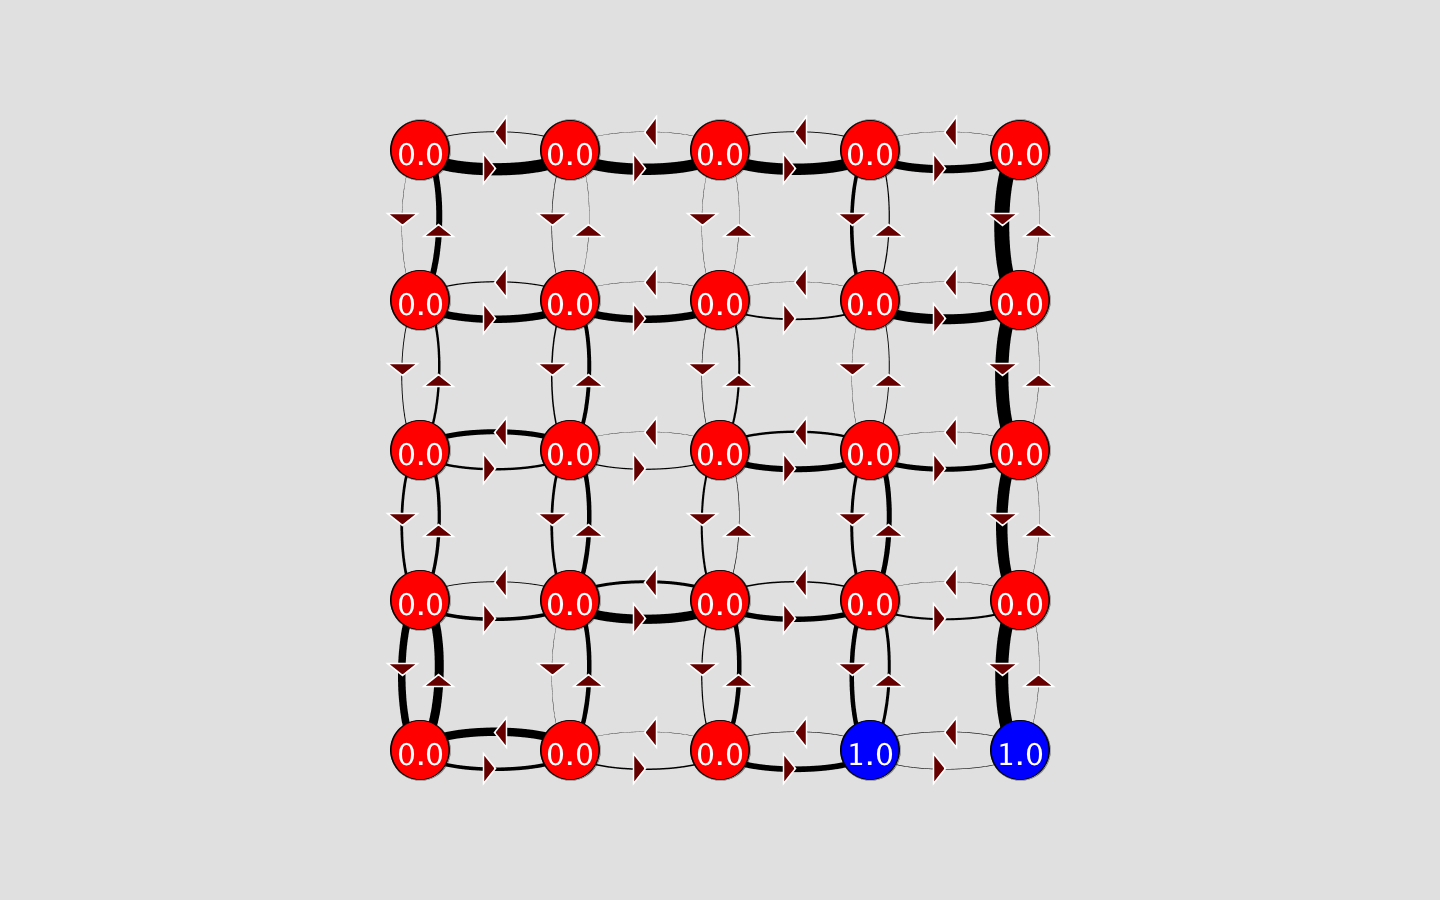
\includegraphics[width=0.9\linewidth]{safetyTestFinal.png}
\end{center}
\caption{Simple $5\!\times\!5$ grid validation test.  The heavier weight
  edges in the figure show higher probabilities.  The thinnest lines
  are generally very near zero but are just drawn to show the
  topology.  The numbers in the nodes are level of safety.  Unless
  otherwise stated, best case of several is shown.}
\label{fig:val1}
\end{figure}

To validate our model we tested that capacity and freeflow constraints
effected our results as expected.  We recorded the path to safety
indicated by highest probabilities calling it the selected path.
We then repeat the experiment by creating a single path from danger to
safety by reducing the freeflow time of the edges along the selected
path, while increasing freeflow along every other edge in the graph
the path is easily found, as it should be.  Similarly, if we increase
maximum capacity along the selected path, while decreasing maximum
capacity along all other edges, the path is again easily found.

We then constructed a maze as seen in Figure \ref{fig:maze}.  The path
indicated in the figure was marked in one test by high capacity and
marked by low freeflow time in the other test.  Notably the safety was
zero except for the safe zone at the end.  Both tests found the easier
routes highlighted in the figure.   As the number of evacuees increases
past the limit of the easy path side streets become used to share the load.

\begin{figure}[h]
\begin{center}
  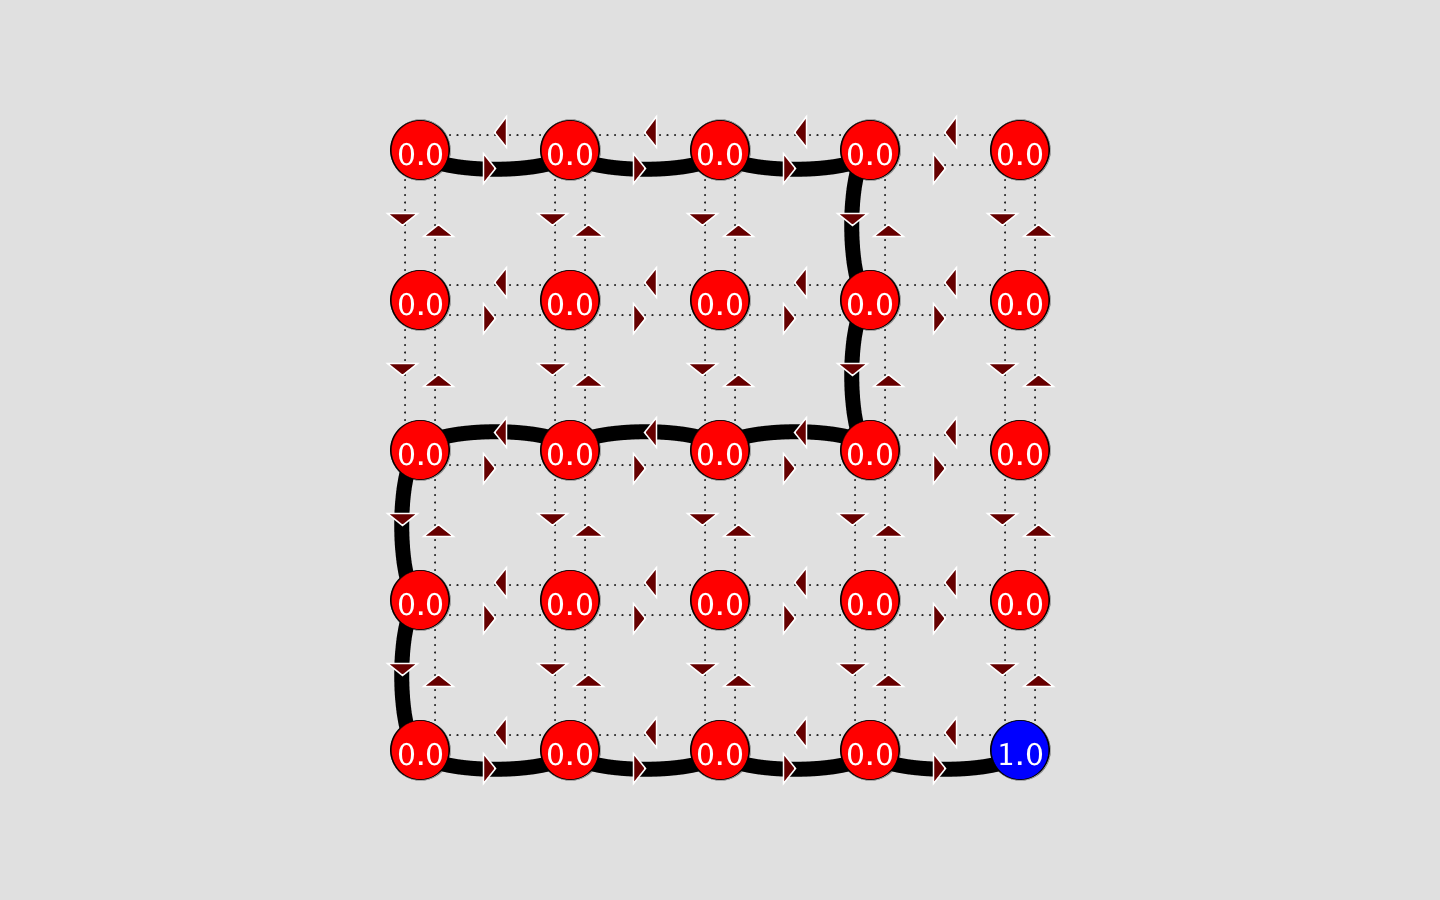
\includegraphics[width=0.9\linewidth]{mazeExemplar.png}
\end{center}
\caption{A cartoon of $5\!\times\!5$ maze test showing the route of least
  resistance.  In this case, these are not a probabilities but rather
  just an indication of where we tried to make the roads faster or
  higher capacity.}
\label{fig:maze}
\end{figure}

\subsection{Dynamic Tests}

The following experiments test if our model accommodates dynamic
events during an evacuation.  We hypothesize that if probability
distributions are optimized in advance, they can be used to initialize
an evolution strategy to reduce optimization time, both in real time,
and number of generations without loss of accuracy.  The results of
these tests demonstrate that pre-optimization leads to faster
adaptability in response to real-time events.  This is a \textbf{very
  important feature} for a real-world evacuation management system.

For these experiments we make several assumptions.  First, we assume
changes are not significantly large.  We assume an algorithm's
population will have genetic contingency information usable for
similar problems.  For example, we assume that from one optimization
to the next during an evacuation, we won't suddenly switch from West
side of the city is safe to East side is safe.  In fact, in such a
case where the graph characteristics have been changed significantly,
re-optimization using a previous solution may take significantly
longer than using random initialization.  The events we are concerned
with are changes in topology, safety zones, capacity, and agent
distribution.

To test our hypothesis, we perform two initial optimizations (case 1)
we optimize a population of solutions that are initialized with random
values for the initial graph configuration and (case 2) we optimize a
population of solutions that are initialized with random values for
the graph configuration after some change in topology, safety,
capacity, or vehicle distribution has been modified.  Finally, (case
3) we use the final population from the first optimization to
initialize the starting population used to optimize the second graph
configuration.  Results will be labeled 1, 2, or 3 corresponding to
the different three cases.  For each test, the evolution parameters
were kept the same for the sake of comparison.  The parameters are
$ES(100+100), P_{crossover}=0.2, P_{mutation}=0.5, \sigma=0.1$

\subsubsection{Adapting to Capacity Changes}

During an evacuation event a roadway may see a change in capacity as a
result of becoming partially blocked by debris, accidents in one or
more lanes on a multi-lane road, or as a result of other unpredictable
events.  In such a case our model must be able to quickly adapt
through re-optimization.  We predict that using pre-optimized traffic
probability distributions will allow for quick adaptation.  To test
this prediction we run three tests.  First, we create a topology with
a maximum capacity of 1000 agents per unit time for all edges,
$G_1$.  Next, we create a topology that is identical, except that
maximum capacity is lowered by 100 for each edge, $G_2$.

We then optimize both of these graphs using our models and record the
average number of generations until maximum fitness is achieved.  We
also store the population of solutions found from $G_1$, as they will
be the starting population for optimization in the next test.  For the
third part of the test we re-optimize $G_2$, starting with the
solutions from $G_1$.  We record and compare the number of generations
needed to reach maximum fitness below.  The probabilities are
graphical represented in Figures \ref{fig:capacity1} and
\ref{fig:capacity2}.  Since the landscape is flat and load is light,
many evacuations plans are equivalent and so variation in the
probabilities occur.  Solution time is shorter in case 3.  Results are
shown Table \ref{tab:tts}.

\begin{figure}[h]
\begin{center}
  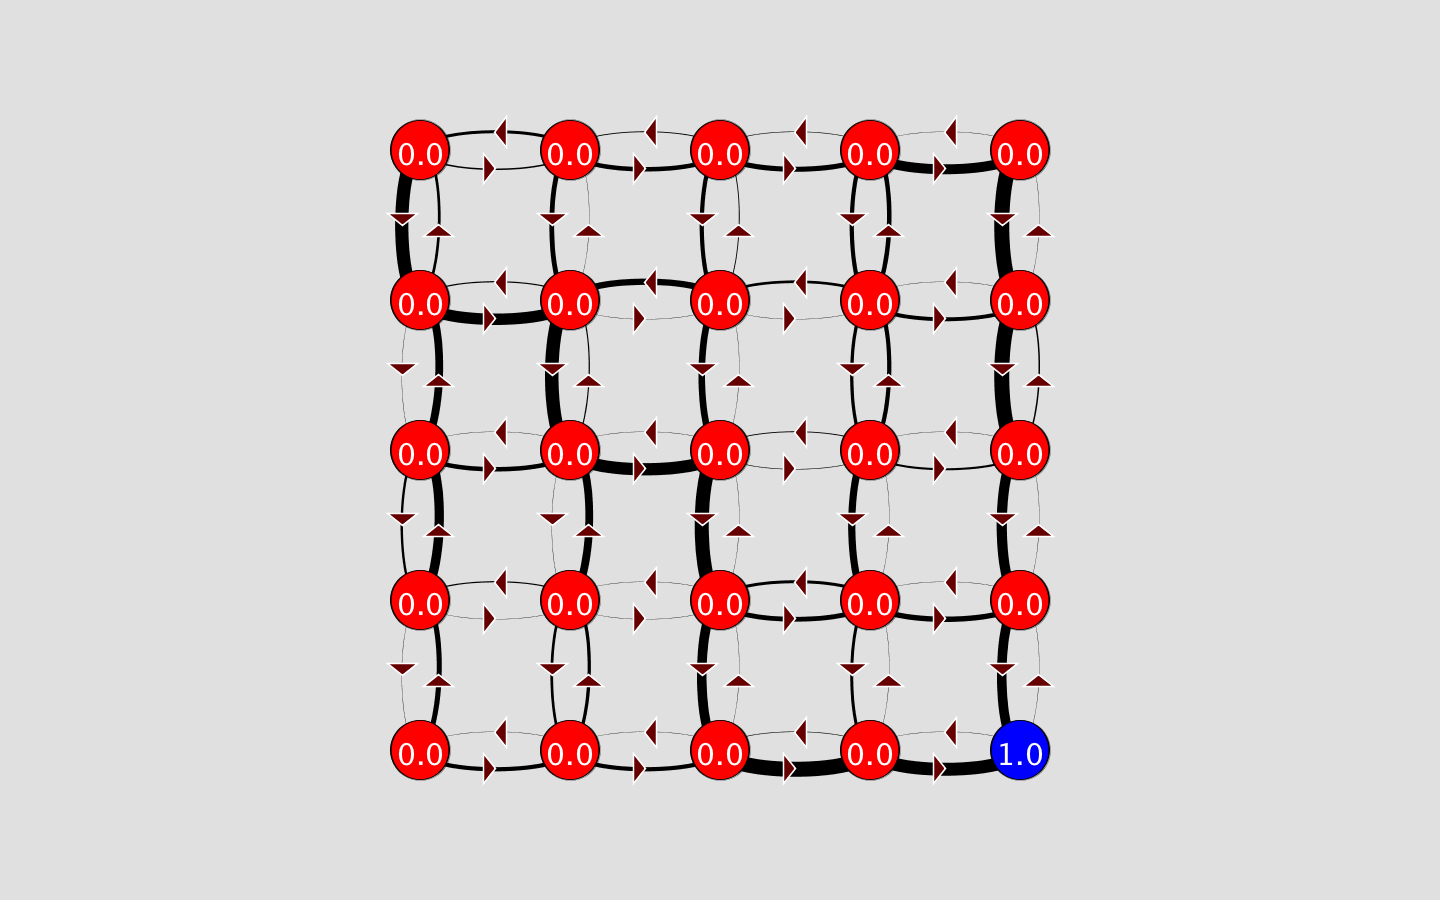
\includegraphics[width=0.9\linewidth]{capacityTestFinal.png}
\end{center}
\caption{$5\!\times\!5$ capacity test results for case 1.}
\label{fig:capacity1}
\end{figure}

\begin{figure}[h]
\begin{center}
  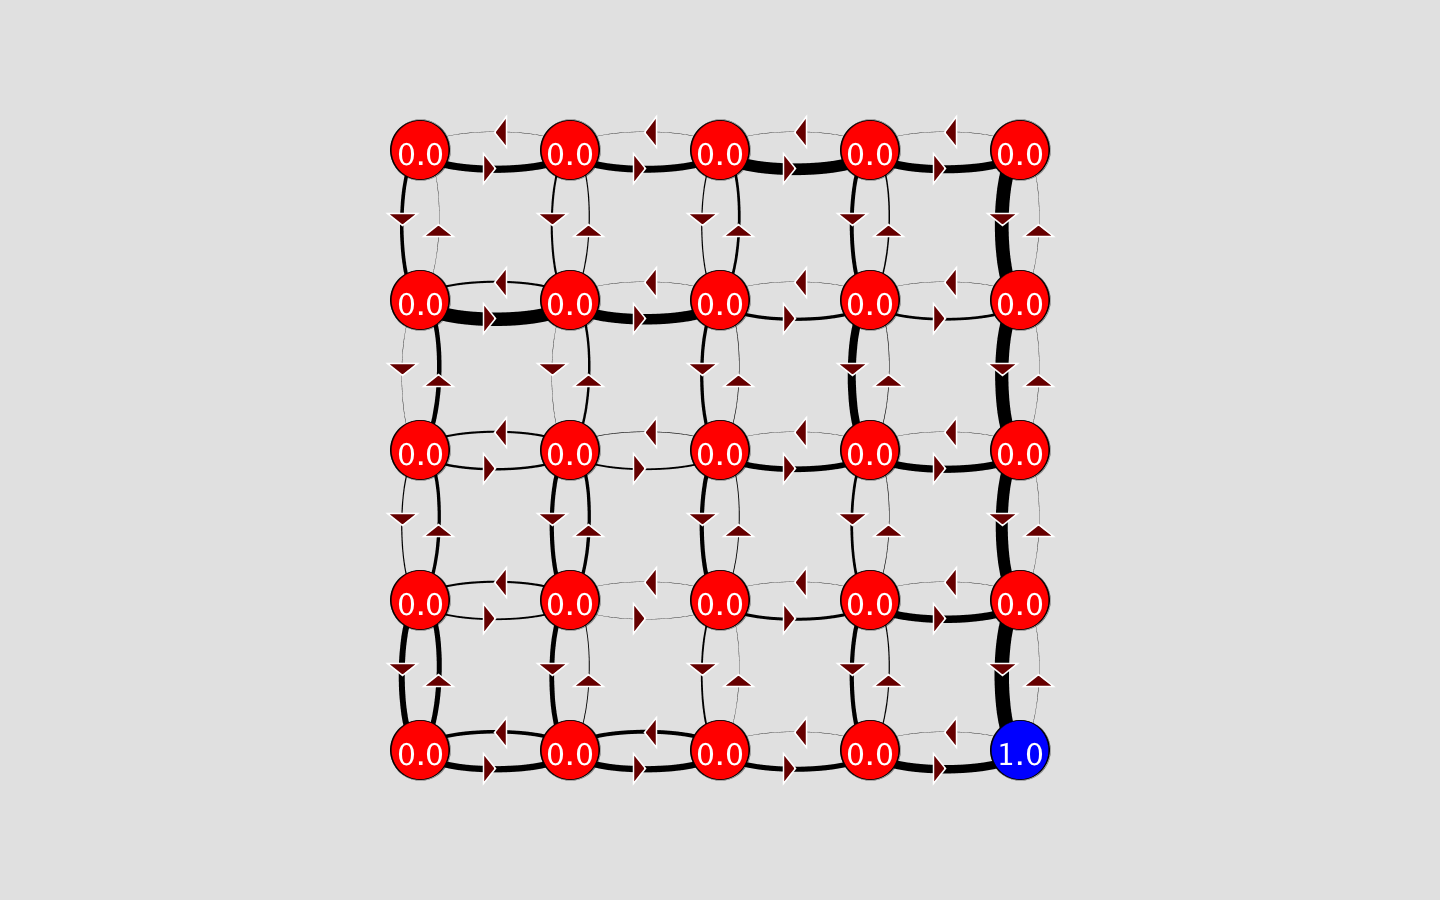
\includegraphics[width=0.9\linewidth]{capacity2TestFinal.png}
\end{center}
\caption{$5\!\times\!5$ capacity test results for case 2.}
\label{fig:capacity2}
\end{figure}


\subsubsection{Adapting to Topology Changes}

Another event that might occur during an evacuation is a change in
topology, meaning some route or partial route becomes unusable, such
as a bridge collapse or a road becoming flooded or completely blocked
by debris.  It is important that our model handles such changes
quickly.  We make a similar prediction to the capacity change test as
well.  Note that a change in topology is a more extreme version of a
change in capacity where maximum capacity is reduced to zero for a
roadway.  We again run three tests but using the bridge topology.  The
first test is on $G_1$, which represents three bridges connecting two
areas, with safety being on the side opposite where vehicles are
started for these tests (See Figure \ref{fig:bridge1}).  $G_2$ for
this test is identical to $G_1$, except with an edge on the center
"bridge" removed representing a collapse.  The first two graphs are
optimized from random traffic assignment probabilities.  We then use
the solutions from the optimization of $G_1$ to optimize $G_2$, and
record the number of generations for comparison (See
\ref{fig:bridge3}).  Results are shown Table \ref{tab:tts}.  Solution
quality is similar but time to solve is substantially shortened.

\begin{figure}[h]
\begin{center}
  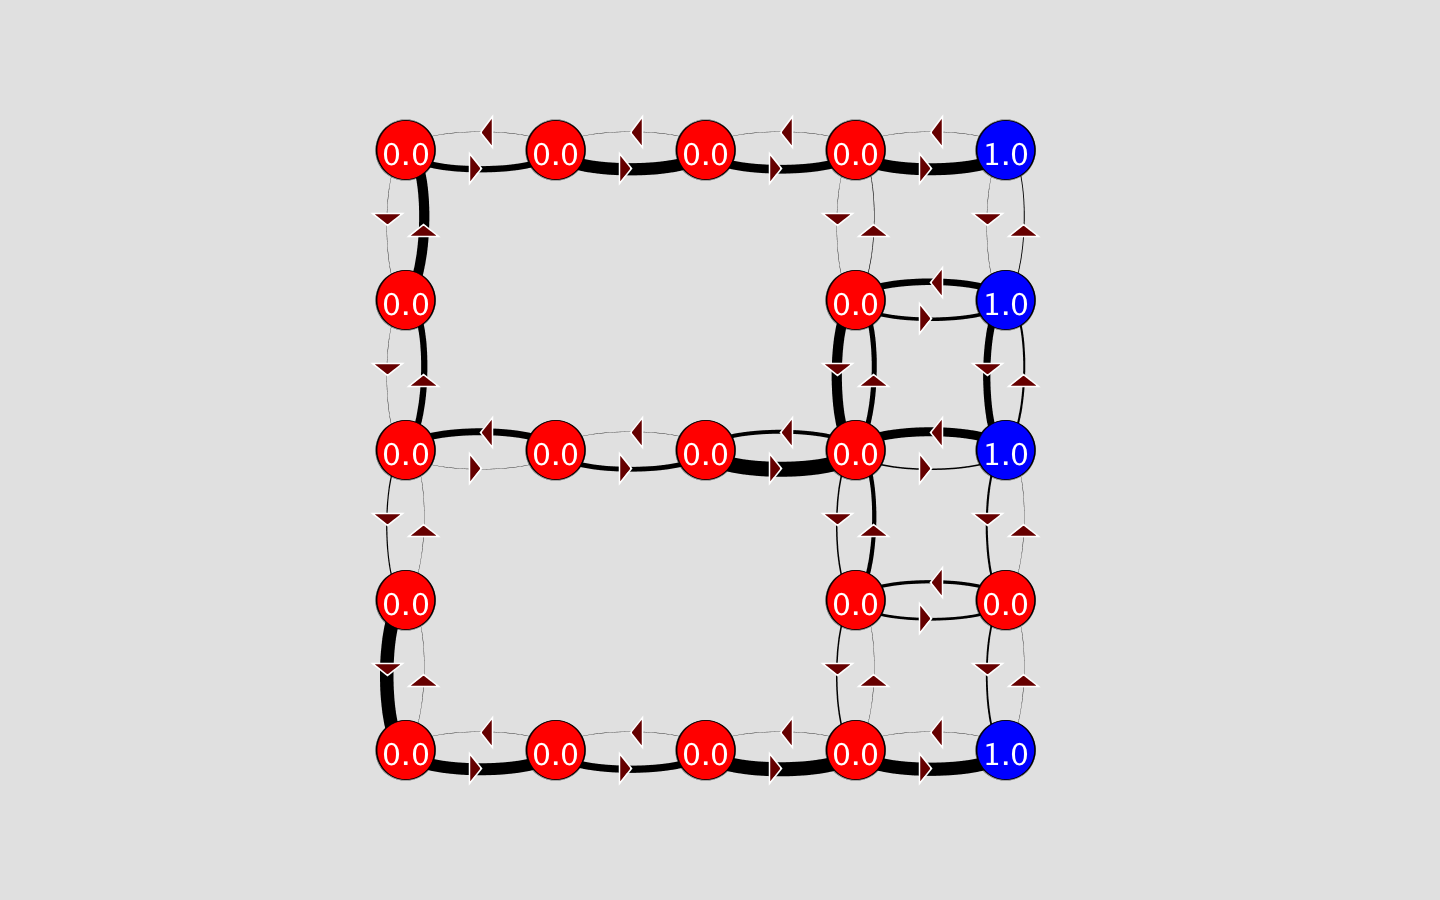
\includegraphics[width=0.9\linewidth]{topologyTestFinal.png}
\end{center}
\caption{The three bridge test.  Probabilities for bridge intact and
random initialization.}
\label{fig:bridge1}
\end{figure}

\begin{figure}[h]
\begin{center}
  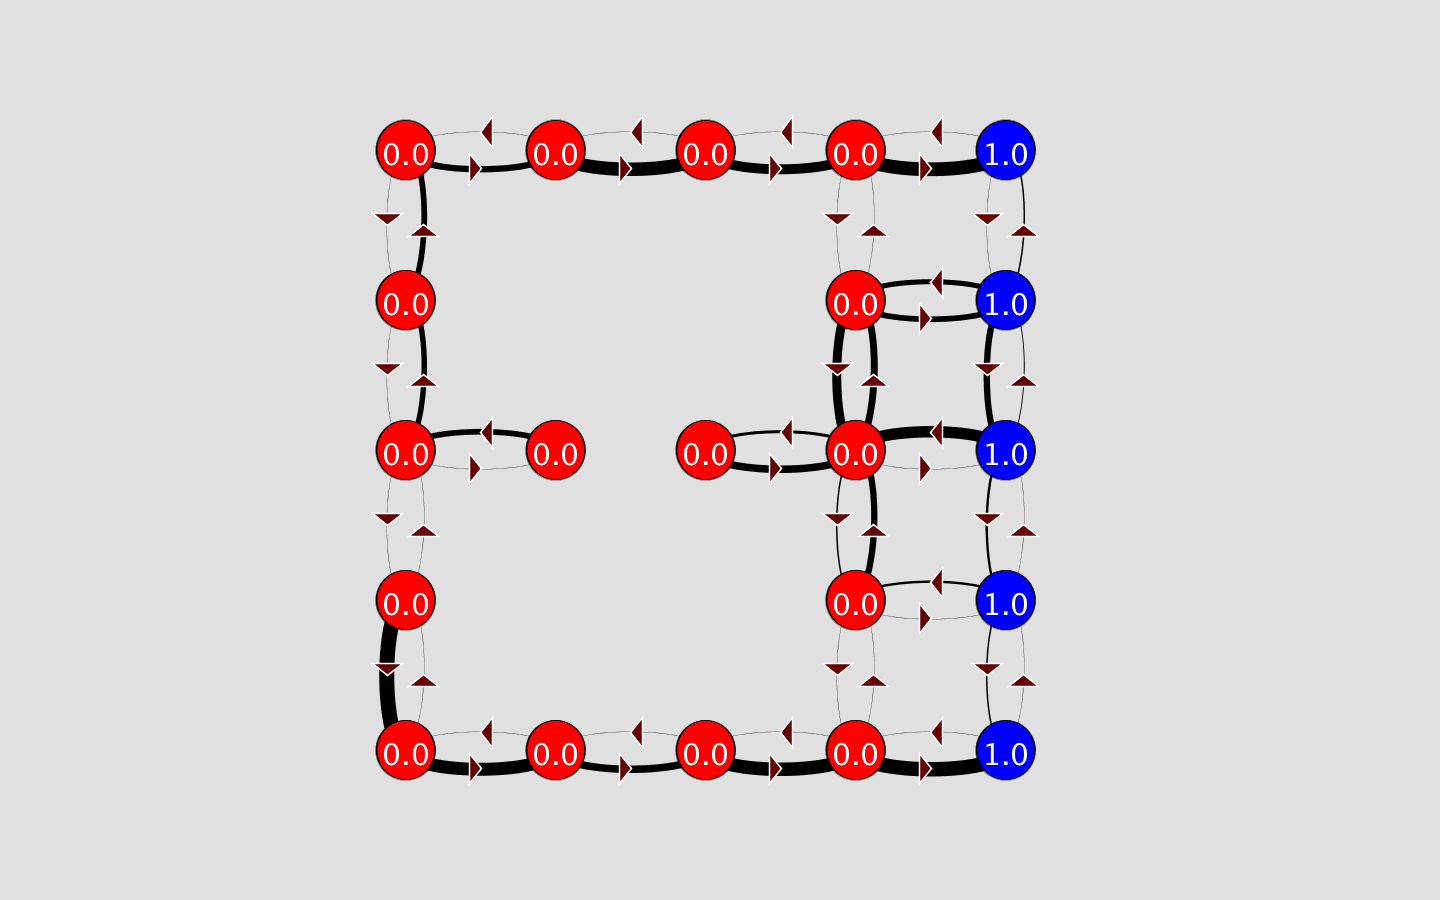
\includegraphics[width=0.9\linewidth]{topology3TestFinal.png}
\end{center}
\caption{The three bridge test.  Probabilities for bridge
  destroyed and population initialized with population from 
previous solution.}
\label{fig:bridge3}
\end{figure}

\subsubsection{Adapting to Agent Distribution Changes}

In an evacuation, it is expected that individual drivers will ignore
evacuation instructions and instead upon arriving at and intersection
rely on their experience driving in the area.  This is expected
because people are under stress and optimal traffic assignments may
produce non-intuitive results in an attempt to balance traffic load on
many streets at once.  In such cases, we must adapt and adjust based
on where vehicles actually are not where we expect them to be.  This
is another reason why it is crucial to continually re-optimize to
adapt to the unforeseen.  We make a similar prediction here - our
model will find an optimal solution faster if initialized with a
pre-computed solution for a similar traffic distribution.  Again, we
use three tests.  All tests use an identical topology, but $G_1$ has
traffic distributed differently than $G_2$.  The first two runs
optimize for different traffic distributions, starting with randomized
traffic assignment probabilities.  The third run uses the optimized
traffic assignment probabilities from the first test, but with the
traffic distribution of the second run.  The traffic probability
distributions are qualitatively not different but the time to solve is
much lower.  Results are shown Table \ref{tab:tts}.

\subsubsection{Adapting to Safety Changes}

During many evacuation events, the threat creating the need for
evacuation is not static.  Examples include hurricanes, floods,
tsunamis, poison gas.  As a result of the dynamic nature of the
threat, it is imperative that our model handles changes in safe areas
quickly.  We predict that our model handles changes in safety quickly,
again provided the change is not too great.  Three runs are used to
perform this experiment.  The first and second are again identical in
topology (see Figure \ref{fig:safety1}).  In the case 3 test the safe
nodes move over one node (see Figure \ref{fig:safety3})..  The
optimized traffic assignment probabilities from run one are used to
initialize the third run, which has safety in the same location as run
two.  Results are shown Table \ref{tab:tts}.   Safety was easily solve quickly.   Perhaps a more difficult safety test will tease out
the difference between case 1 and 3 for this problem.

\begin{figure}[h]
\begin{center}
  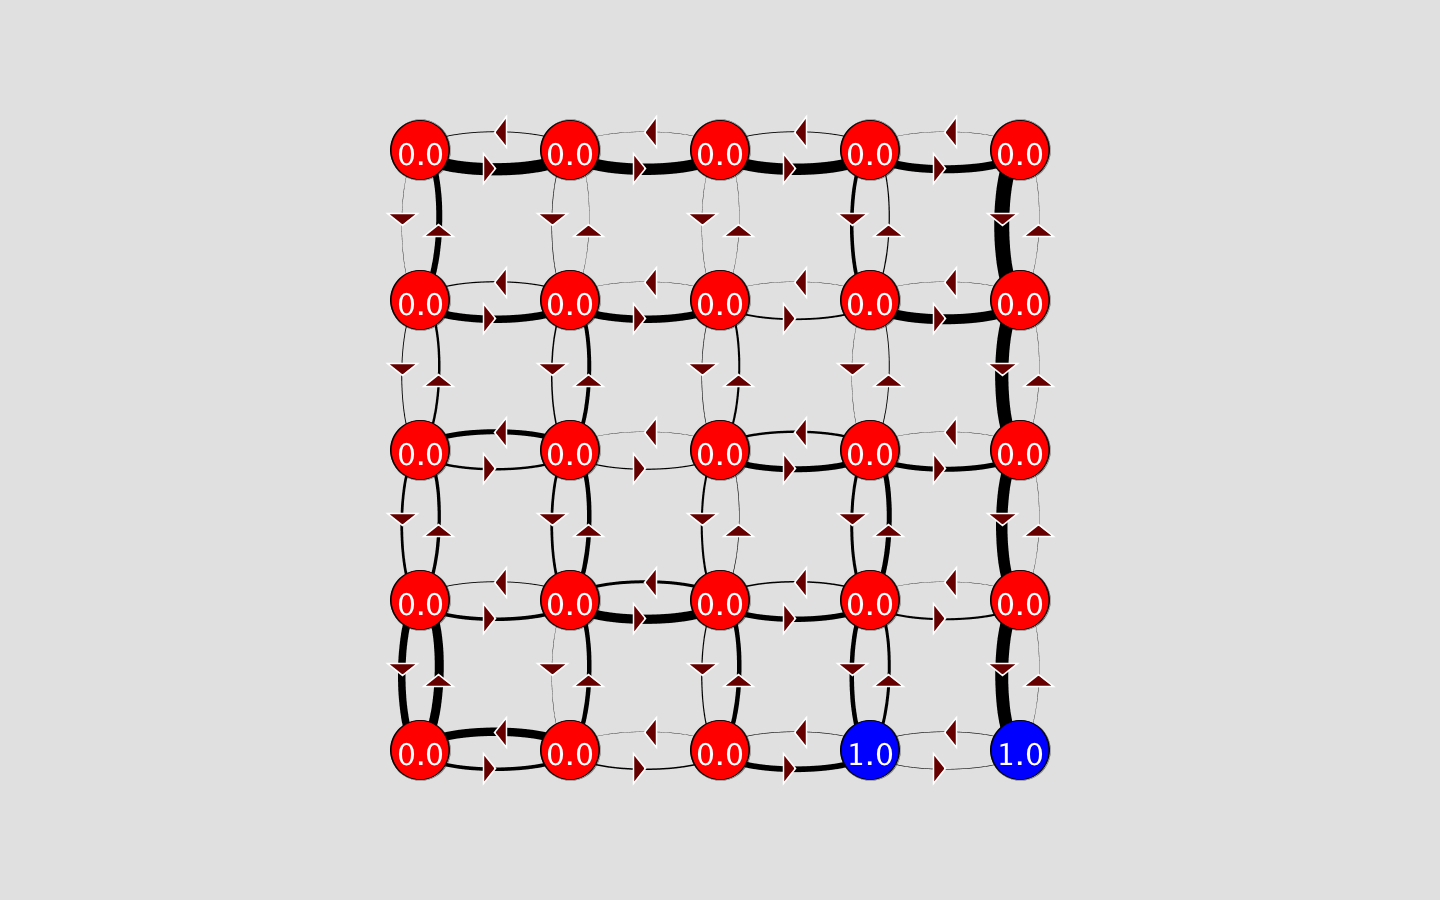
\includegraphics[width=0.9\linewidth]{safetyTestFinal.png}
\end{center}
\caption{$5\!\times\!5$ safety test for case 1.}
\label{fig:safety1}
\end{figure}

\begin{figure}[h]
\begin{center}
  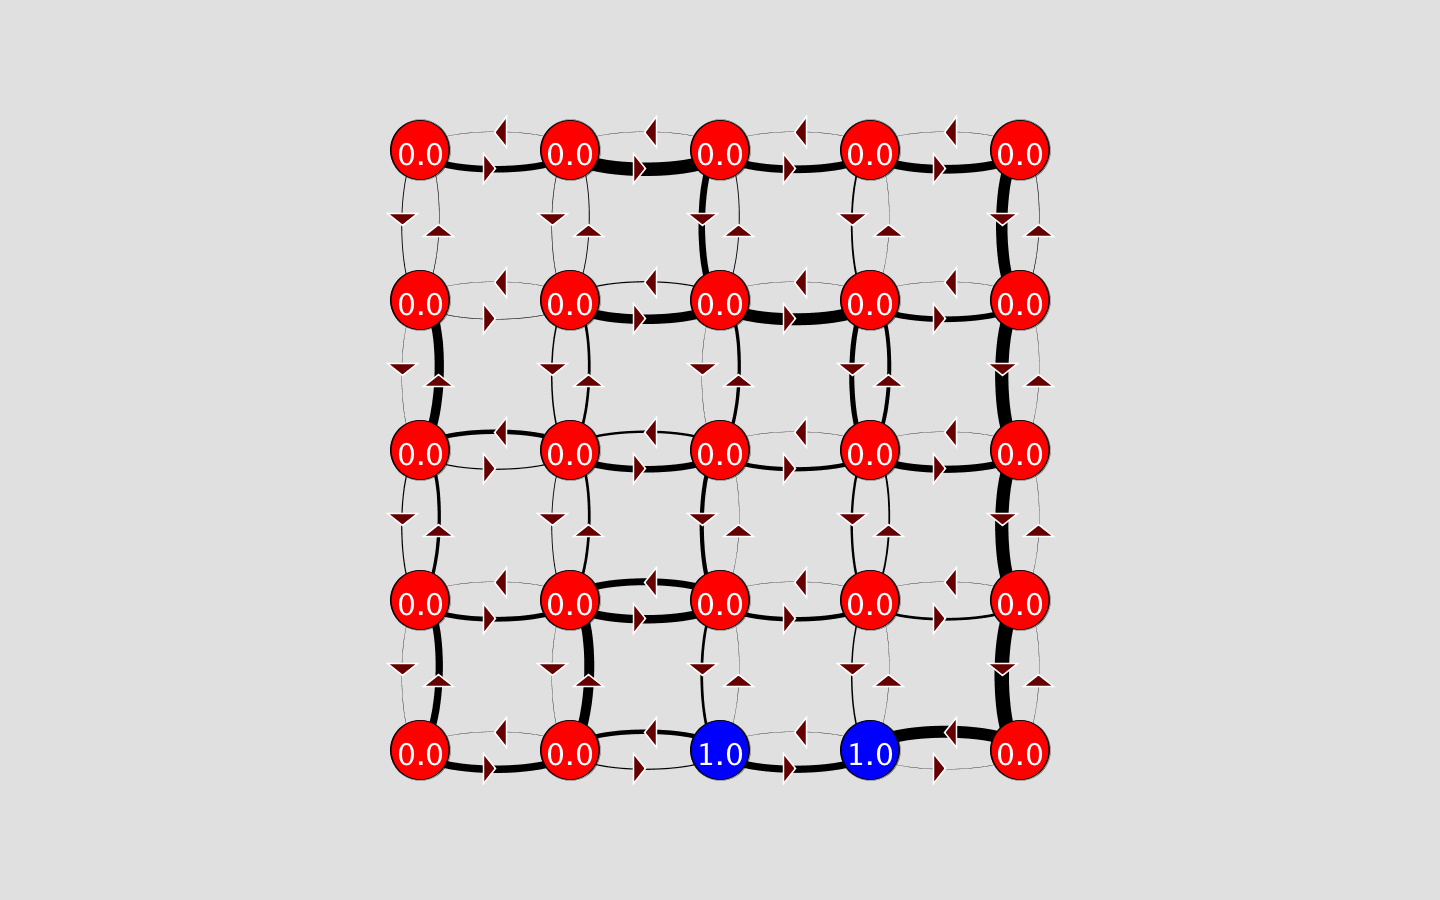
\includegraphics[width=0.9\linewidth]{safety3TestFinal.png}
\end{center}
\caption{$5\!\times\!5$ safety test for case 3.}
\label{fig:safety3}
\end{figure}

\begin{table}
  \begin{center}
    \caption{Time to Complete Optimizations in Dynamic Tests: Agents,
      Capacity, Safety, and Topology.  In all cases the suffix numbers
      1, 2, or 3 represent the three cases in each of the dynamic
      tests.  100 runs of each case were performed.  ``Gens'' is
      generations and $t_{hours}$ is duration of simulation.  }
\label{tab:tts}
\begin{tabular}{l|cc|cc|c}
\hline \hline
Test & Avg. Gens & $\sigma_{Gens}$ & Avg. Fit & $\sigma_{fit}$ & $t_{hours}$ \\
\hline
Capacity1 & 47.75 & 5.208 & 1.0 & 0.0 & 1.0 \\
Capacity2 & 55.1 & 6.64 & 1.0 & 0.0 & 1.0 \\
Capacity3 & 4.35 & 2.19 & 1.0 & 0.0 & 1.0 \\
\hline
Topology1 & 73.54 & 15.835 & 1.0 & 0.001 & 0.5 \\
Topology2 & 69.92 & 13.9 & 0.998 & 0.009 & 0.5 \\
Topology3 & 7.01 & 4.574 & 1.0 & 0.0 & 0.5 \\
\hline
Agents1 & 77.99 & 9.605 & 0.999 & 0.003 & 0.7 \\
Agents2 & 89.69 & 8.577 & 0.998 & 0.004 & 0.7 \\
Agents3 & 30.5 & 8.325 & 1.0 & 0.0 & 0.7 \\
\hline
Safety1 & 1 & 1 & 1.0 & 0 & 1.0 \\
Safety2 & 1 & 1 & 1.0 & 0 & 1.0 \\
Safety3 & 1 & 1 & 1.0 & 0 & 1.0 \\
\hline
\end{tabular}
  \end{center}
  \end{table}

\begin{figure}[h]
\begin{center}
  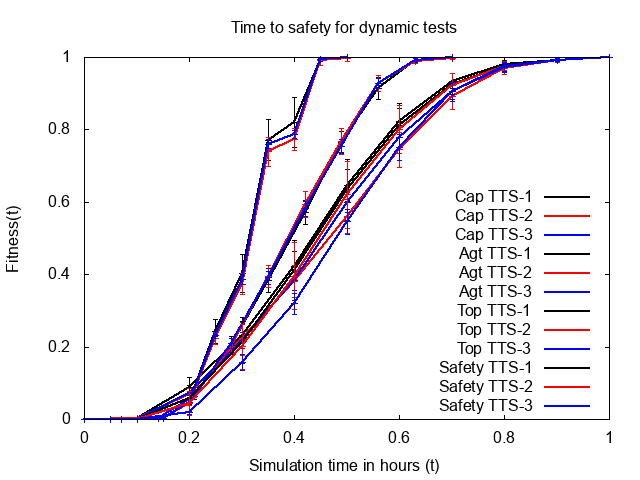
\includegraphics[width=0.9\linewidth]{composite-tts-graph.png}
\end{center}
\caption{A comparison of the quality of answers for the four dynamic
  tests.  This indicates the answers are of comparable quality.}
\label{fig:comptts}
\end{figure}
  

\begin{figure}
\centering
\begin{tabular}{cc}
\subfigure[Capacity]{
  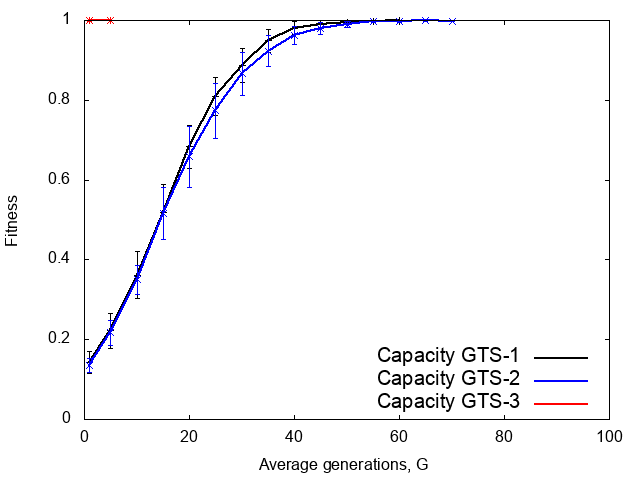
\includegraphics[width=0.47\linewidth]{capacity-gts.png}}
&
\subfigure[Topology]{
  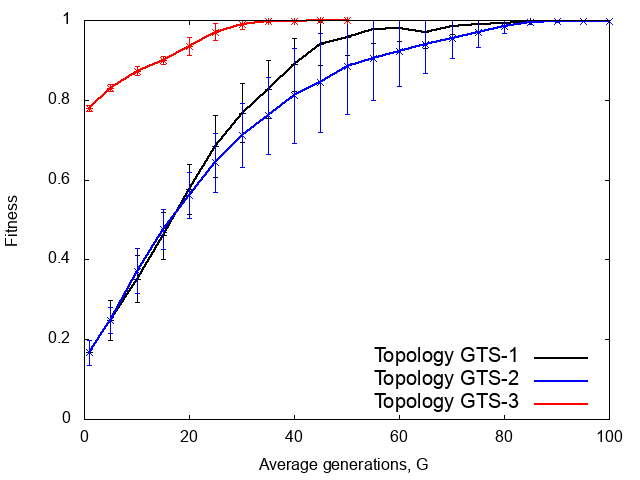
\includegraphics[width=0.47\linewidth]{topology-gts.png}} \\
\subfigure[Agents]{
  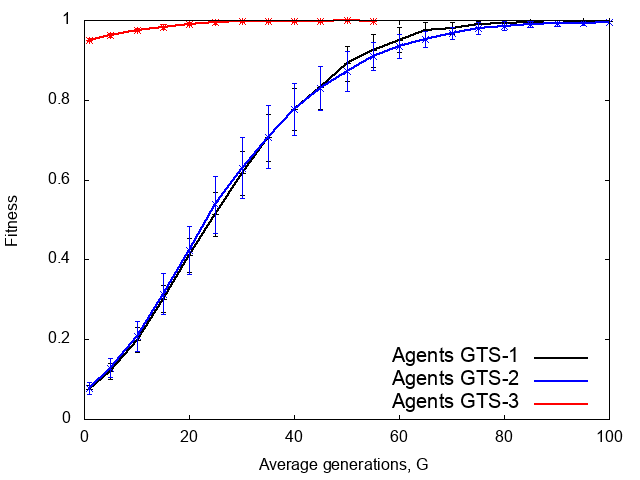
\includegraphics[width=0.47\linewidth]{agents-gts.png}} 
&
\subfigure[Safety]{
  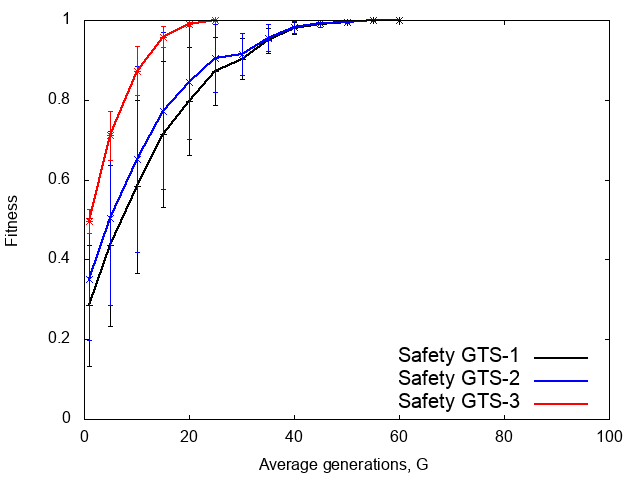
\includegraphics[width=0.47\linewidth]{safety-gts.png}} \\
\end{tabular}
\caption{The speed of solution for the four dynamic tests and across
  cases 1, 2, and 3.  Generations along X-axis and fitness along
  Y-axes.  Values averaged over 100 runs.}
\label{fig:dynspeed}
\end{figure}

\subsubsection{Summary}

In the dynamic tests we adjusted one of four attributes to represent
events that can change a transportation network in an evacuation.
Graphs shown in Figure \ref{fig:dynspeed} show that priming the
population with a population that produced a successful solution for
the pre-event problem produces a solution more quickly than just
starting the optimization over.  Figure \ref{fig:comptts} shows the
quality of the answers is substantially the same.  We believe that as
long as the change is modest the population contains ``contingency
gene'' that will help speed the adaption to the new problem.  These
results are encouraging but we are following with more focused tests
in our future work.

\subsection{Comparison Tests}

Here we compare our results to results of other tests found in the
literature and suited to our model.  Specifically, we borrow the test
problem found in Bazzan et al.  \cite{bazzan2014evolutionary}.  In
their paper, Bazzan et al.  seek to minimize average travel time by
evolving traffic assignments through a graph, given a set of vehicles,
origin/destination pairs for those vehicles, and a set of $k$ shortest
paths.  They use a classic graph from \cite{willumson2001transport},
(see Figure \ref{fig:baz}) with the freeflow times specified.  The way
we model capacity is different, but comparable.  We seek to compare
our results to provide some context of how our model holds up compared
to other work.

\begin{figure}[h]
\begin{center}
  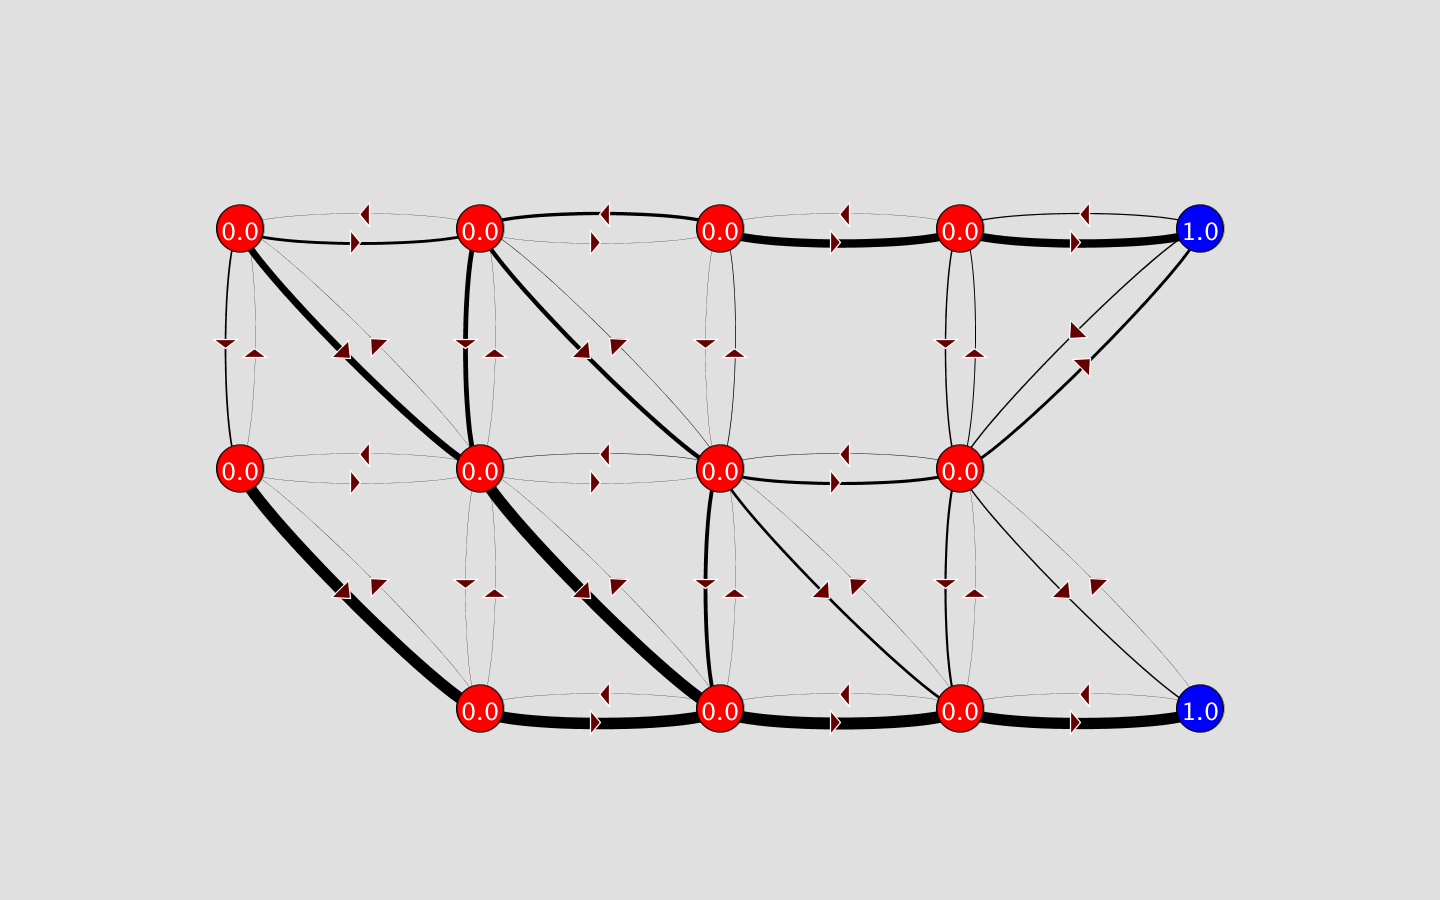
\includegraphics[width=0.9\linewidth]{bazzan-2.png}
\end{center}
\caption{The network from Bazzan et al. 2014.}
\label{fig:baz}
\end{figure}

In their experiment they run $k$ origin/destination pairs, with $k$
ranging from 2 to 16.  We choose to compare to the case where $k=4$.
We run our experiment with two vehicle origin nodes, corresponding to
their origins, with two safe nodes, corresponding to their
destinations.  We let our model optimize for safety, and provide the
results and comparison below.

Our model is not as optimal, and our average time to complete all
traffic is significantly lower.  This is probably due to an
inconsistency in modeling, but is an area for future study and
analysis.  While our model does find routes to safety, the routes
found are not as fast as those found by Bazzan et al.
The average time to safety (TTS), with standard deviation is show
in Figure \ref{fig:bazperf}.

\begin{figure}[h]
\begin{center}
  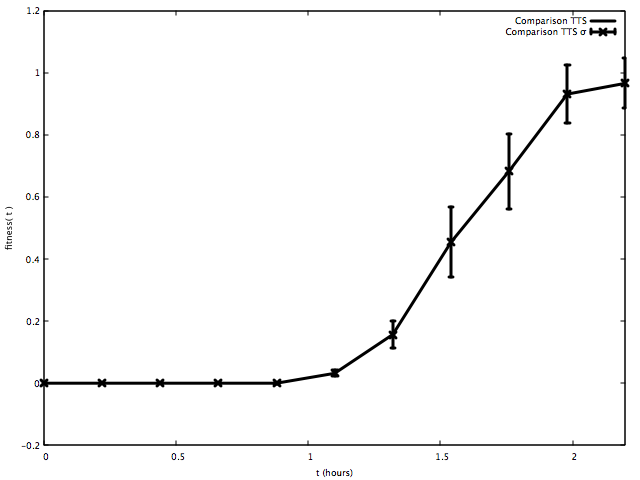
\includegraphics[width=.9 \linewidth]{bazzan-tts-graph.png}
\end{center}
\caption{Performance of our algorithm on the Bazzan test averaged over
100 trials.}
\label{fig:bazperf}
\end{figure}



\subsection{Scaling Tests}

To test the ability of our model to handle real-world urban evacuation
problems we used traffic model data for Boise, Idaho, a city with
approximately 650,000 people.  As the data we used was less precise
than we would like, some assumptions and liberties were taken.  First,
we don't know the exact freeflow rates of all the roads, nor the
maximum capacities of each roadway.  However, our goal is to discover
how long it takes to optimize solutions for a large problems with
large numbers of vehicles.  Our data includes 283 nodes, and 457
edges.  These do not represent every road and intersection, but rather
many of the artery roads and feeders (see Figure \ref{fig:boise}).  We
believe the vast majority of the evacuee's time will be spent on these
roads and so the test is a realistic estimation of evacuation time.
We tested a number of cases with varying numbers of vehicles and
groups.  Each test has a group of ten vehicles initialized to start at
every node in the graph.  These agents are placed here to ensure
probabilities at every area of the graph are optimized.  In our model,
if an area of the graph sees no traffic, the probabilities at that
area are not punished or rewarded which produces random traffic
probabilities.  This affect could have dangerous results in real-world
application.  The tests we run for Boise start with only the single
groups of ten vehicles at each node, and scale up to 102,830 vehicles,
with large grouping.  Each test is run with identical evolution and
graph values, except where the vehicles are initialized.  Vehicle
initialization is random, except for a set of vehicles forced to start
in each node.  Each test was run 10 times and the time to run averaged
over those runs.  These tests were performed with a simulation time of
one hour.  The results are found in Table \ref{tab:boise}.

\begin{figure}[h]
\begin{center}
  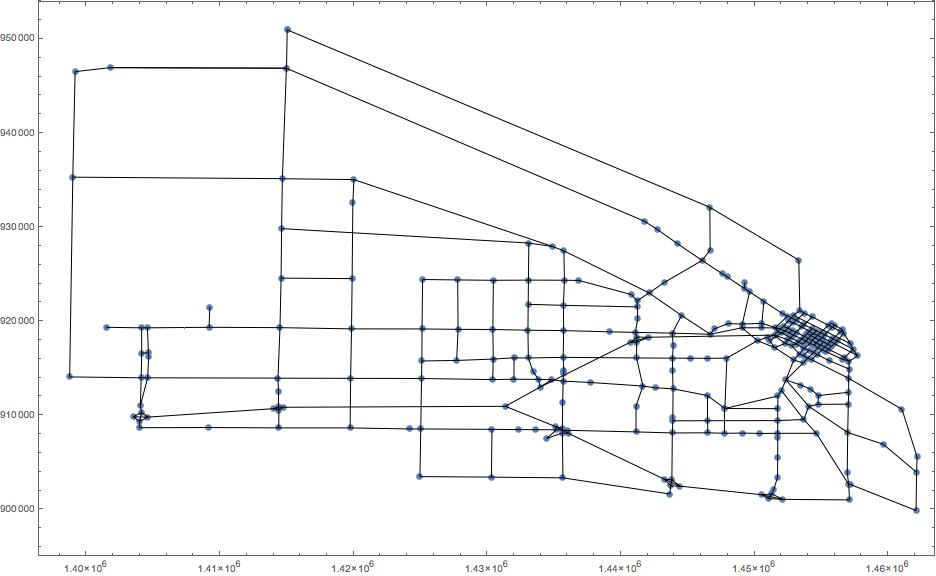
\includegraphics[width=0.9\linewidth]{boise.png}
\end{center}
\caption{The Boise Transportation Network.  Notice the dense packed
  streets in the downtown area.  The map is of an area approximately
  ten miles wide.}
\label{fig:boise}
\end{figure}

\begin{table}
  \begin{center}
    \caption{Time to solve the Boise problem.  Individuals is the
      total number of individuals.  Rand Groups is the number of
      randomly placed groups throughout the city above the groups that
      are evenly distributed across the 283 nodes of the city.  Group
      size is the number of individuals in each group or agent.  It
      defines the grouping of the agents For timing the runs were
      performed using Centos Linux system running on 2.4 GHz Intel
      Xeon X56xx processors.}
\label{tab:boise}
\begin{tabular}{l*{4}{c}}
  \hline \hline
  Individuals & Rand Groups & Group Size & Run Time (min)  \\
  \hline
2,830     & 0    & 10   & 3.5        \\
2,930     & 10   & 10   & 3.28       \\
3,830     & 10   & 100  & 3.5        \\
12,830    & 100  & 100  & 4.4        \\
102,830   & 100  & 1000 & 4.25       \\
1,002,830 & 1000 & 1000 & 19.05      \\
  \hline
\end{tabular}
  \end{center}
  \end{table}

\subsection{Future Work}

These experiments showed the feasibility of
using a cloud of probabilities and an ES algorithm
to solve a wide variety of evacuation problems.
We have added node capacities which creates another
level of practical constraint on the problem and are
working on a wide variety of disaster management
problems.

\section{Conclusions}

In conclusion, we have evolved static probability distributions that
are shown to provide routing to safe areas in reasonable time.
Further, the solutions used are provided as initializations for
evacuation parameter changes, which reduce the optimization times of
the updated scenarios.  This makes an evolution based real-time
continuous optimization of an evacuation feasibile.  The main
advantages of our proposed model includes a robust method for adapting
to the dynamic conditions of a real disaster, relatively fast
computation time, and robustness achieved through both evolution and a
vehicle distribution model, instead of a more ridged point-to-point
routing for individual agents.

\section{Acknowledgments}

This material is based in part upon work supported by the
National Science Foundation under Cooperative Agreement
No.  DBI-0939454.  Any opinions, findings, and conclusions or
recommendations expressed in this material are those of the
author(s) and do not necessarily reflect the views of the
National Science Foundation.  We thank Michigan State faculty
member Dr. Kalyanmoy Deb for his collaboration in this research.
\pagebreak
\bibliography{mybib}
\bibliographystyle{IEEEtran}
\end{document}
